\RequirePackage[l2tabu, orthodox]{nag}
\documentclass{article}

\usepackage[letterpaper, margin=1.3cm]{geometry}
\usepackage{siunitx}
\usepackage{mathtools}
\usepackage{multicol}
\usepackage{amssymb}
\usepackage{mathrsfs}
\usepackage{enumitem}
\usepackage{circuitikz}
\usepackage{booktabs}
\usepackage{multirow}
\usepackage{pdfpages}
\usepackage[outputdir=obj]{minted}

\ctikzset{
    logic ports=ieee,
    logic ports/scale=0.7,
}

\title{ECE 410 Assignment 4}
\author{Michael Kwok}

\begin{document}
\maketitle

\begin{enumerate}
  \item A possible algorithm to debounce this switch would be to count up to a set number \(n\) of ``stable'' readings before that value is set every \(t\) seconds. Once the counter reaches the value of \(n\), the read value of the switch will be set to either on or off depending on the values read.

  \item A potential advantage for using different edges for the modules would be that a higher clock speed can be achieved since the datapath could be set at the falling edge, while the controller is selecting memory addresses and such at the rising edge. The delay between the rising and falling edge could be used as setup time for the datapath.

        A major disadvantage is that the system would be harder to design reliably and reason about. Timing analysis would also become more complex as the system does different things at each edge, and so more things need to be put under consideration when trying to calculate the timings in the system.

        The advantages do not outweigh the disadvantages as nowadays systems are extremely complex, and reliability should be a bigger concern over speed. The performance increase is also likely to be very small, making the entire exercise not worth the larger mental load.

  \item A rectangular mesh network could be easier to manufacture than an H-tree clock network due to using simple lines as the mesh. A disadvantage would be that due to the shape, the propagation delay for the clock might not be as uniform as the H-tree, and different devices will get clocked slightly off relative to each other.

  \item Last 2 questions attached at the end
\end{enumerate}

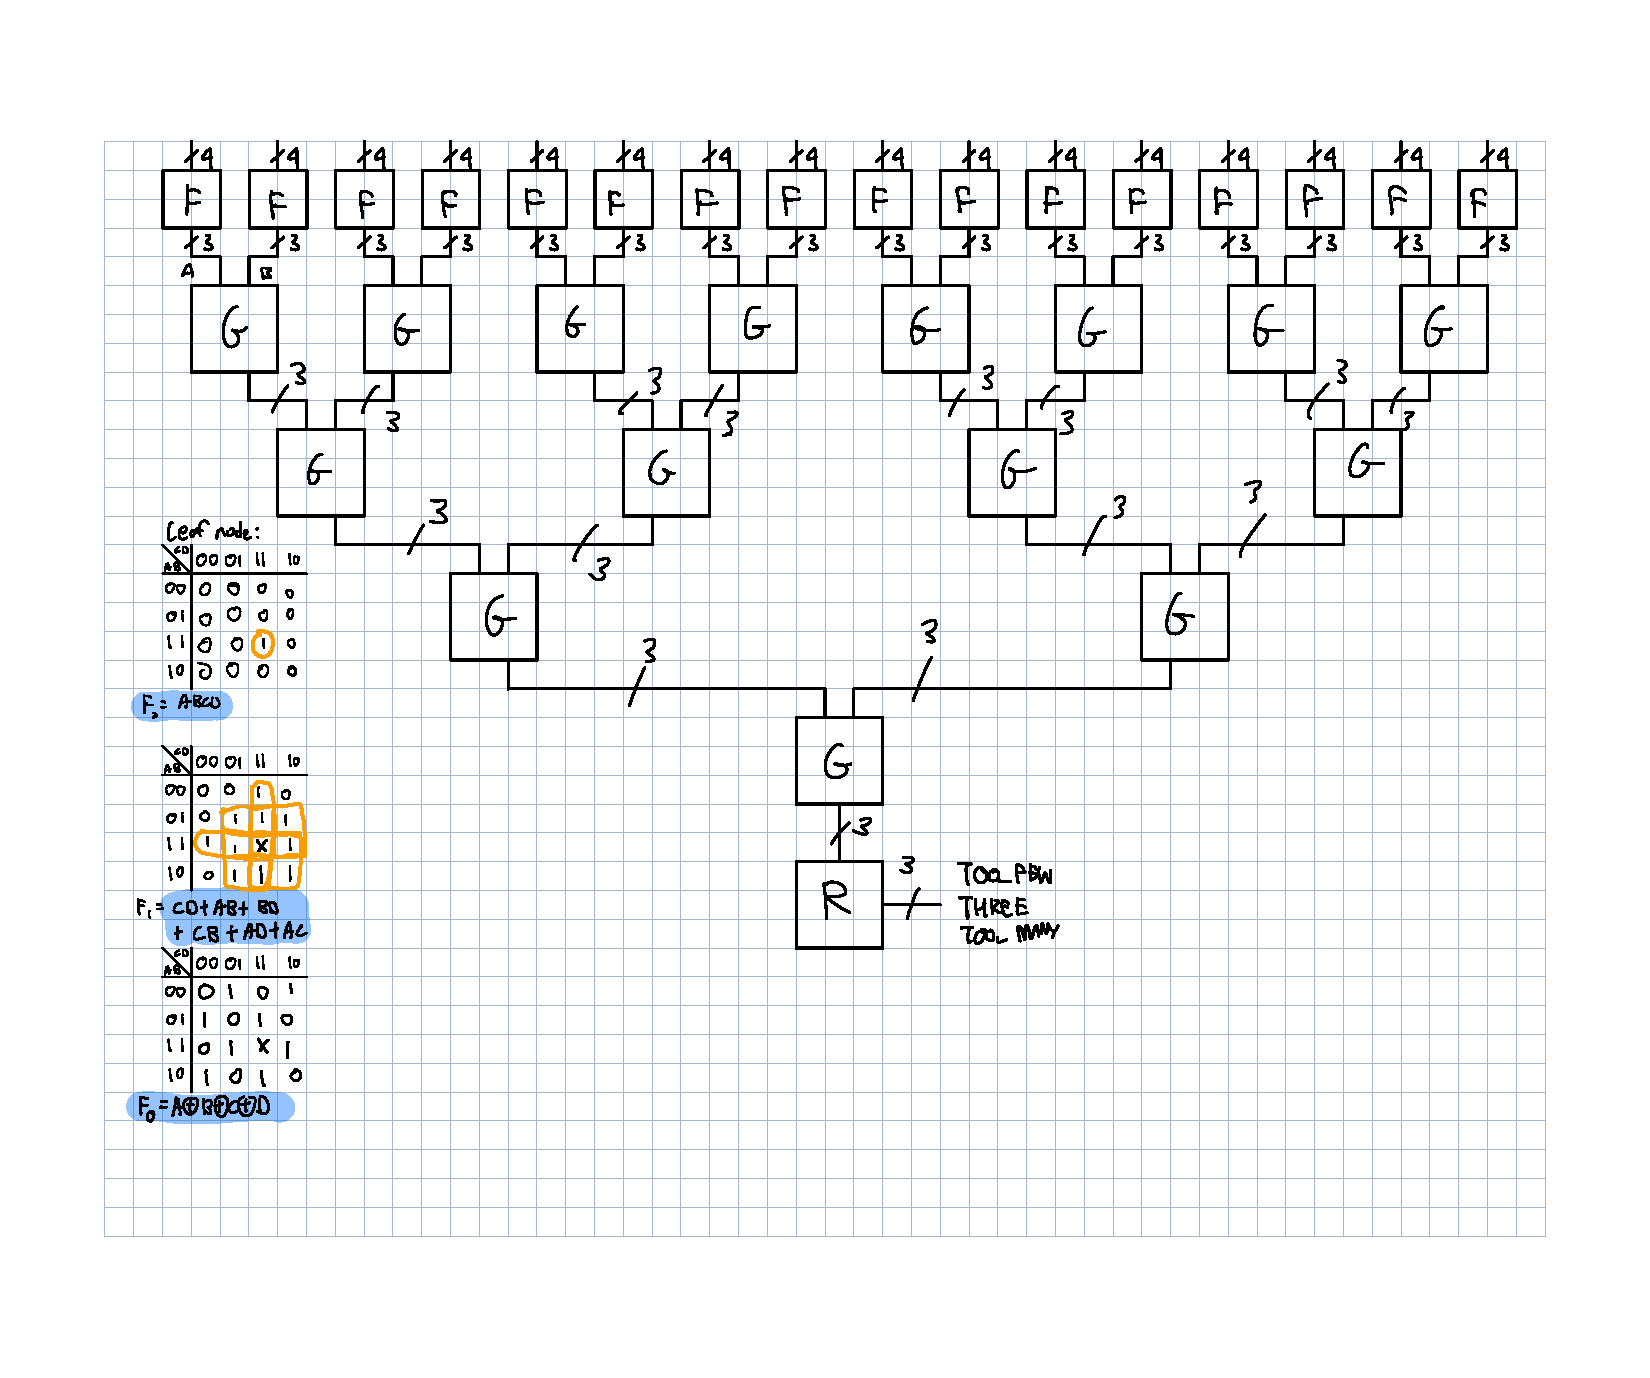
\includepdf[pages={-},fitpaper,rotateoversize]{Diagrams.pdf}

\end{document}
